\section{Scattering Spectrometer}
\label{sec:scatteringspectrometer}

\subsection{Detector layout}

\begin{itemize}
    \item Motivations for new design: dependence of neutrino flux from the radius, reduced area free from background muons 
    \item Description of \emph{One magnet} design (Figure \ref{fig:spectro_layout})
    \item \emph{One magnet} option VS \emph{Two magnets} option


\begin{figure}[htbp]
\centering
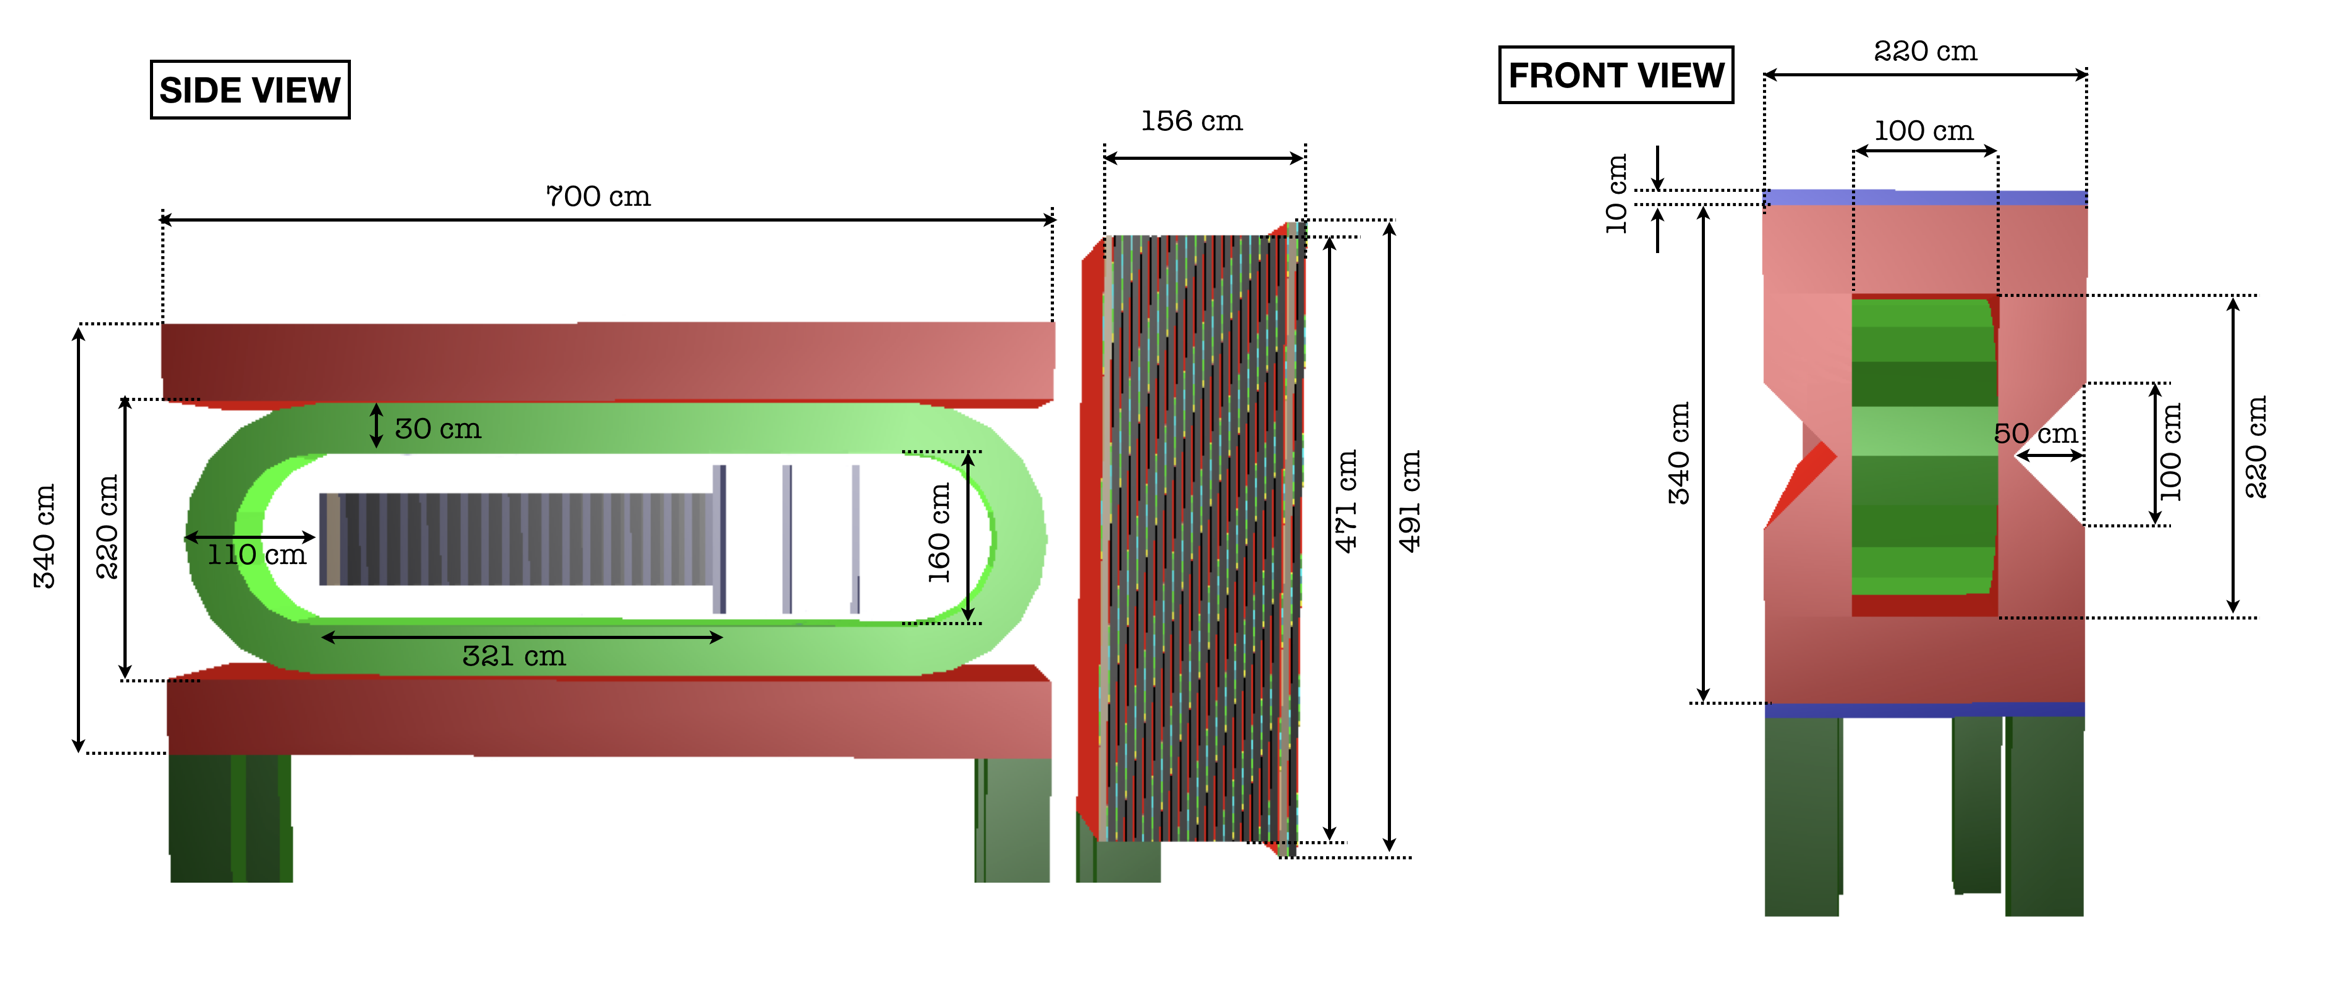
\includegraphics[scale=0.35]{figs/ScatteringSpectrometer/ScatteringSpectro.png}
\caption{Layout of the Scattering Spectrometer}
\label{fig:spectro_layout}
\end{figure}

\item Magnet design
 \begin{itemize}
 \item[$\circ$] Main constraints: inner volume and cross-section, 1.2 T uniform magnetic field, saturation field in iron, access to inner detector
 \item[$\circ$] Description of the magnet layout (Figure \ref{fig:magnet_layout})
 \end{itemize}
 

\begin{figure}[htbp]
\centering
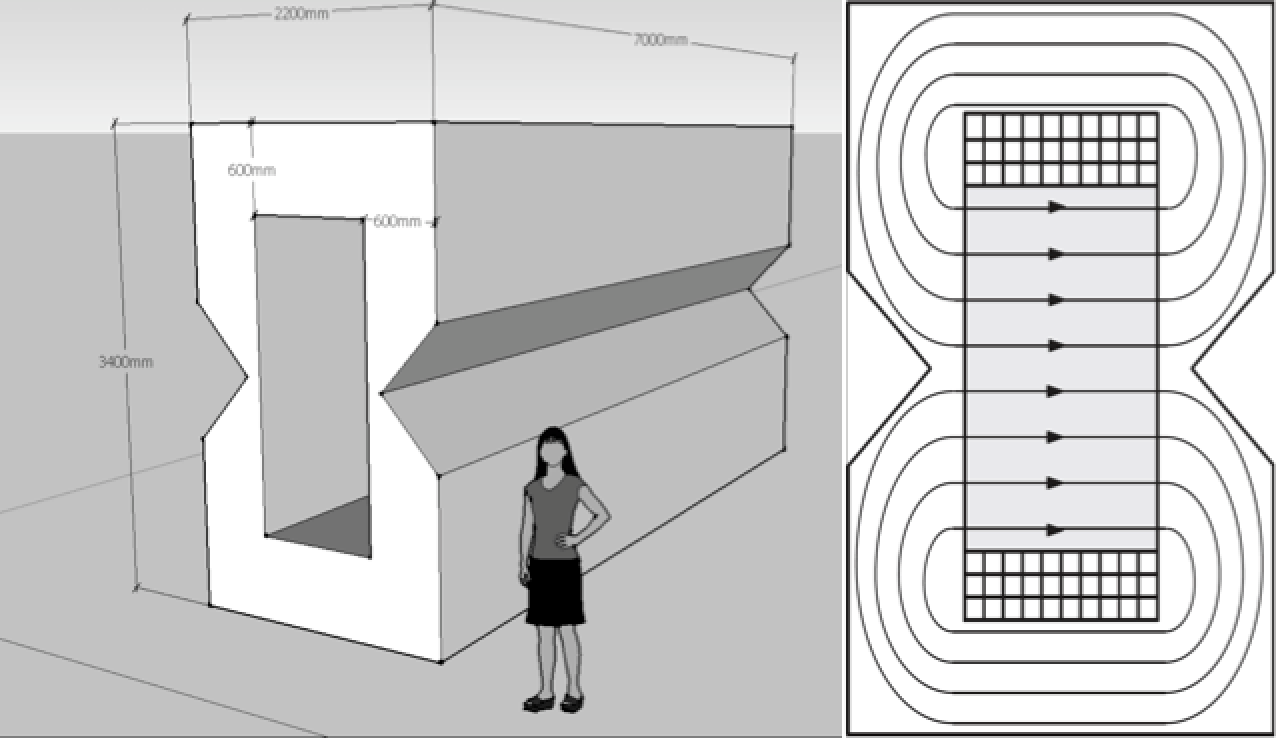
\includegraphics[scale=0.35]{figs/ScatteringSpectrometer/ScatteringSpectroMagnet.png}
\caption{Layout of the Scattering Spectrometer Magnet}
\label{fig:magnet_layout}
\end{figure}

\item Emulsion Target 
\begin{itemize}
    \item[$\circ$] Emulsion Cloud Chamber
    \item[$\circ$] Compact Emulsion Spectrometer: results from 2017 Test Beam
\end{itemize}

\item Target Trackers
\begin{itemize}
    \item[$\circ$] Requirements
    \item[$\circ$] Options under investigation: gas detectors (results from 2017 Test Beam), SciFi
\end{itemize}

\item Magnetic Spectrometer
\begin{itemize}
    \item[$\circ$] Requirements
    \item[$\circ$] Option under investigation: SciFi
\end{itemize}

\item Muon Filter
\begin{itemize}
    \item[$\circ$] Requirements
    \item[$\circ$] Detector layout
\end{itemize}

  \end{itemize}
  
\subsection{Neutrino detection}
\begin{itemize}
    \item Track reconstruction and primary vertex identification
    \item Decay search
    \item Charge measurement 
    \item Momentum measurement
    \item Particle identification in the Muon Filter
    \item Overall detection efficiency for different $\tau$ decay channels
\end{itemize}

\begin{figure}[htbp]
\centering
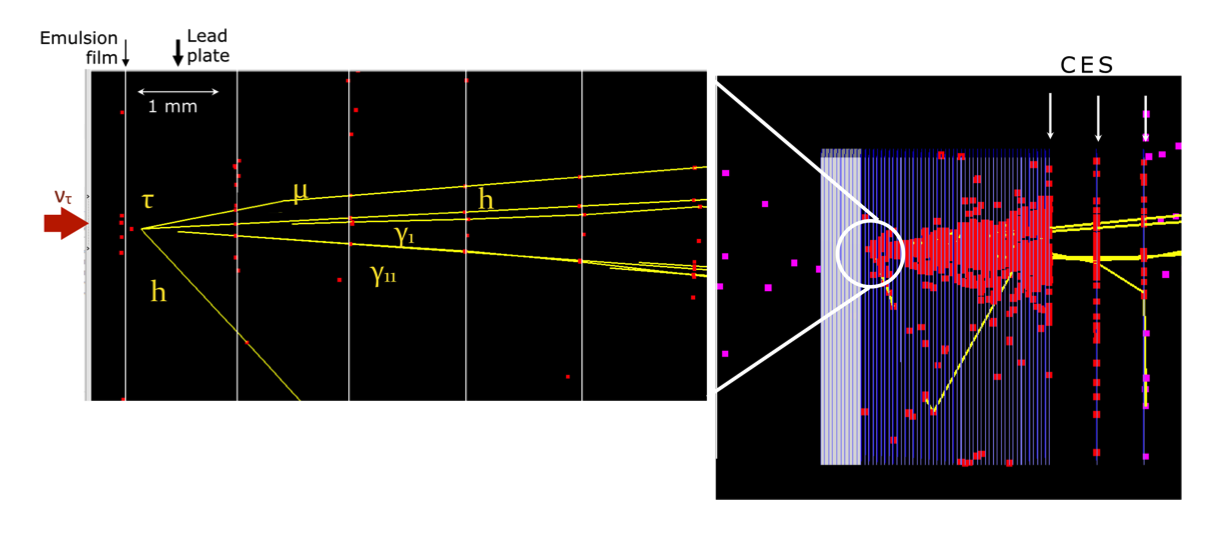
\includegraphics[scale=0.5]{figs/ScatteringSpectrometer/NeutrinoRecEmu.png}
\caption{$\nu_\tau$ interaction and subsequent $\tau \to \mu$ decay in the Emulsion Target.}
\label{fig:neutrino_rec_emu}
\end{figure}

\begin{figure}[htbp]
\centering
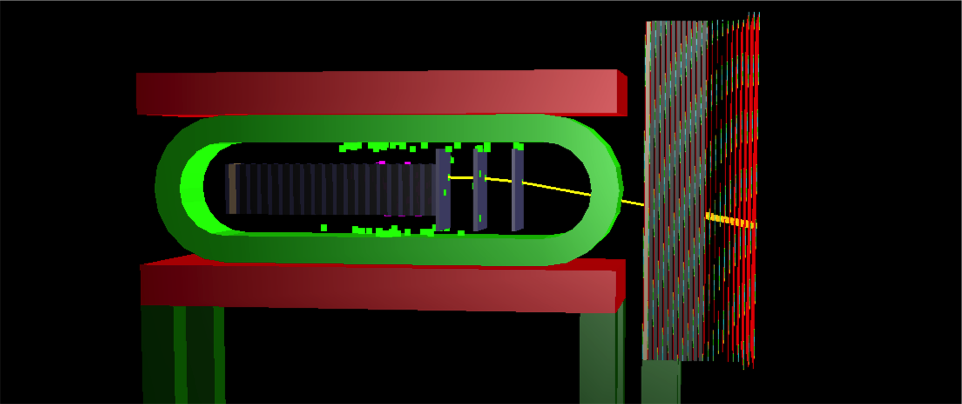
\includegraphics[scale=0.5]{figs/ScatteringSpectrometer/NeutrinoRecAll.png}
\caption{$\nu_\tau$ interaction and subsequent $\tau \to \mu$ decay in the Scattering Spectrometer.}
\label{fig:neutrino_rec_all}
\end{figure}

\subsection{Electromagnetic shower identification}
\begin{itemize}
    \item Pattern recognition (Figure \ref{fig:shower_id})
    \item Energy resolution (Figure \ref{fig:shower_res})
    \item Pointing accuracy 
\end{itemize}

\begin{figure}[htbp]
\centering
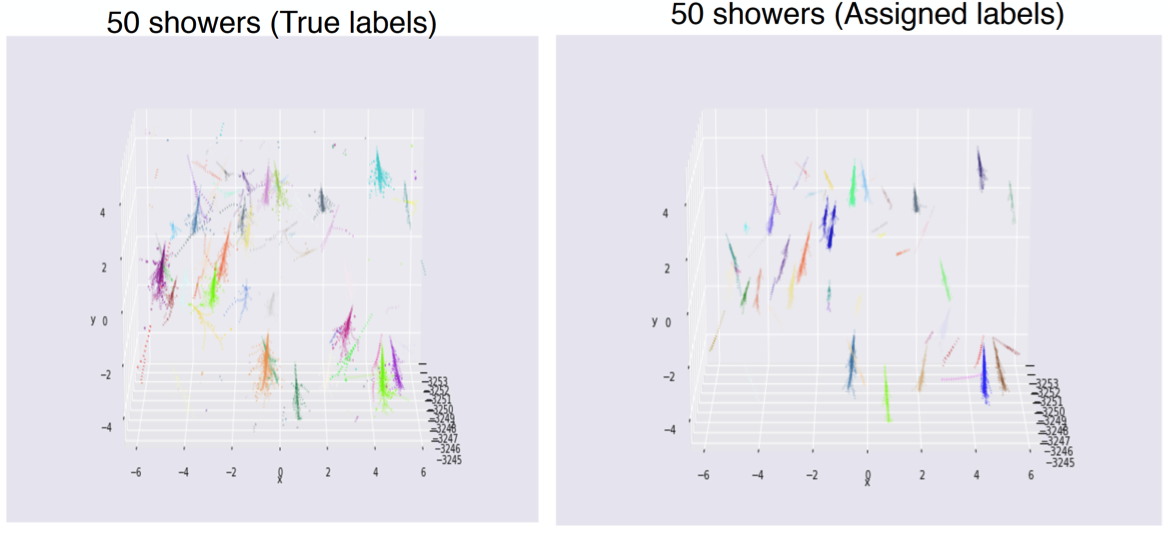
\includegraphics[scale=0.6]{figs/ScatteringSpectrometer/Showers.png}
\caption{Electromagnetic shower identification in the ECC.}
\label{fig:shower_id}
\end{figure}

\begin{figure}[htbp]
\centering
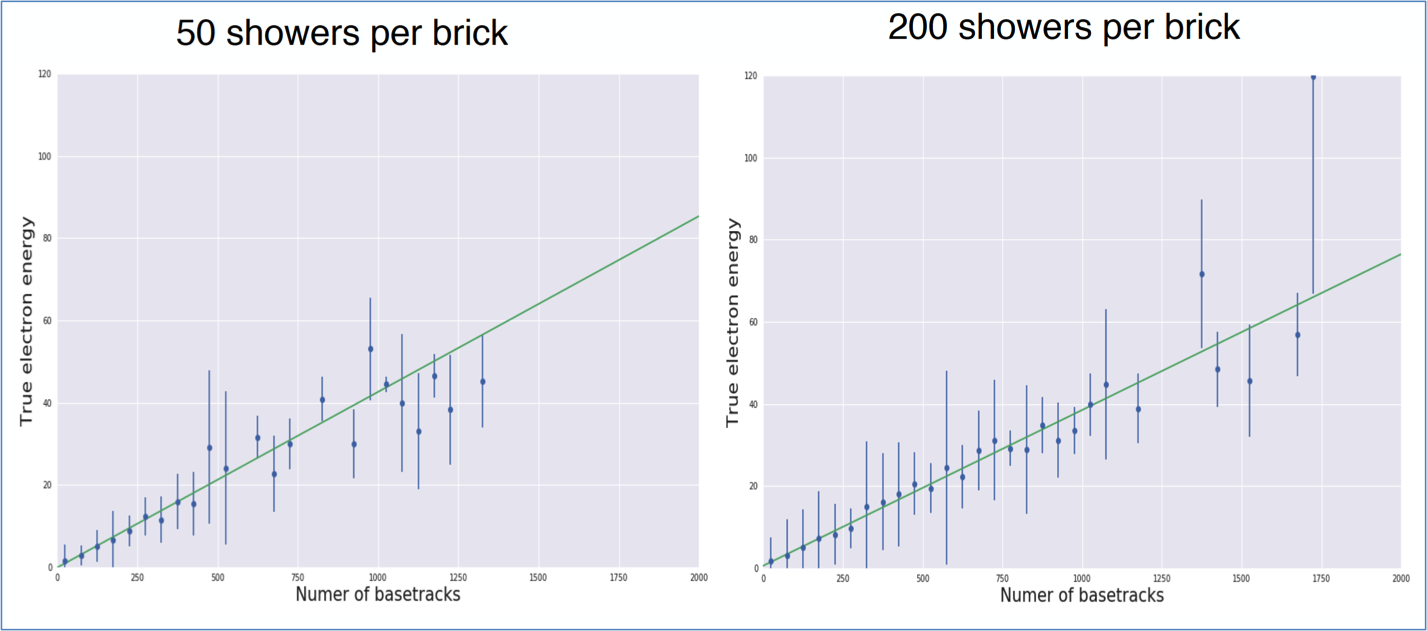
\includegraphics[scale=0.5]{figs/ScatteringSpectrometer/ShowersRes.png}
\caption{Energy resolution of electromagnetic showers in the ECC.}
\label{fig:shower_res}
\end{figure}

\subsection{Timing performances}

\subsection{Combined performances of TT and ECC/CES}
